\chapter{Prototypische Anwendung}
\label{cha:prototypische_anwendung}

Im folgenden Kapitel wird eine Applikation entwickelt, welche die in Kapitel \ref{cha:hybrid_cloud_architektur} ab Seite
\pageref{cha:hybrid_cloud_architektur} erarbeitete Hybrid-Cloud-Architektur prototypisch implementiert.

Dafür wird ein Web-Frontend erstellt, welches die in einer Datenbank vorliegenden Informationen visualisiert. Bei den
Daten handelt es sich einerseits um statische Werte wie Vorname, Nachname, usw. als auch um dynamische Werte wie zum
Beispiel ein Kundenwert, der in einem Diagramm dargestellt werden soll.

Zur Umsetzung wird neben einer Laufzeitumgebung für das Frontend auch der Service Text\-2Speech in Bluemix eingerichtet.
Die erstellte Laufzeitumgebung und der Service werden im Anschluss miteinander verbunden, damit diese Daten über die
VCAP-Variaben austauschen können.

Den Zugriff auf die Daten in der Datenbank ermöglicht eine COBOL-Anwendung, welche nicht näher beschrieben oder definiert
ist. Dies bedeutet, dass es keine Informationen über Schnittstellen oder der genaue Funktionsweise der Anwendung gibt.
Eine Analyse der Schnittstellen und Funktionen erfolgt durch das Tool \textit{IBM Application Discovery}.

Nachdem die Schnittstellen der COBOL-Anwendung definiert sind, wird ein Java-Wrapper geschrieben, welcher eine
REST-Schnittstelle zur Verfügung stellt. Diese kann genutzt werden, um Daten aus der Datenbank über die COBOL-Anwendung
zu erhalten. Die Kommunikation zwischen dem Java-Wrapper und COBOL-Anwendung erfolgt durch die Schnittstelle \textit{WOLA}.

Da die COBOL-Anwendung nicht alle Informationen aus der Datenbank liefert, wird zusätzlich der DB2 Rest Service sowie ein
Machine Learning (Watson)-Service genutzt.

Wie in \cite{online_einleitung_app} zu lesen, spielt für viele Firmen neben einer vernünftigen Webseite auch eine
Smartphone-App eine immer wichtigere Rolle. Aus diesem Grund wird im nächsten Schritt sowohl eine Android- als auch eine
iOS-App erstellt.

Diese stellen ebenfalls die Informationen aus der Datenbank dar und sollen sich für den leichten Umstieg hinsichtlich
Funktion und Design, wenn überhaupt, nur gering von dem Web-Frontend unterscheiden.

Die Kommunikation zwischen Frontend, Android- und iOS-App und dem Backend auf dem Mainframe erfolgt durch
den Secure Gateway-Service in Bluemix.

Eine grobe, schematische Übersicht über die zu implementierende Anwendung ist in Abbildung \ref{fig:architektur_clouduebersicht}
auf der Seite \pageref{fig:architektur_clouduebersicht} zu sehen.

\begin{figure}[h]
  \centering
    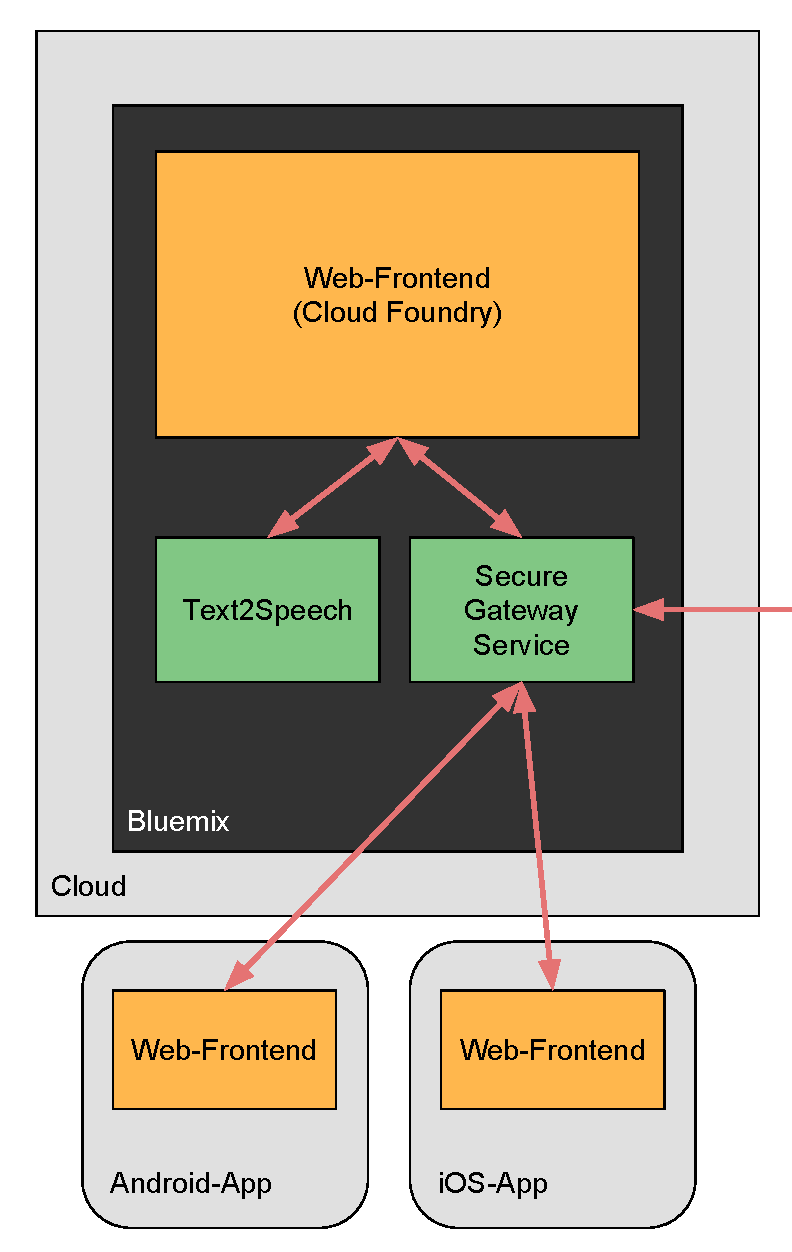
\includegraphics[scale=0.5]{images/kapitel_4/architektur_clouduebersicht.pdf}
  \caption{Grobe Übersicht über die Prototypische Anwendung}
  \label{fig:architektur_clouduebersicht}
\end{figure}